\section{Erweiterungen}\label{sec:erweiterung}

\textbf{Einsatzleitung:} Die Darstellung der Einsatzleitung ist ebenfalls \autoref{fig:feed-objekt} zu entnehmen.
In dem in dieser Abbildung gezeigten Objekt liegt die Objektleitung beim Finanzamt.
Die Darstellung ist der klassischen Version nachempfunden, welche bereits in \autoref{sec:feedbackPerson} erklärt wurde.

Die momentane Darstellung ist jedoch nicht final.
Sie ist nur für Menschen mit konkretem Fachwissen zugänglich und sollte im Laufe der Zeit durch eine auch für Laien verständliche Version ersetzt werden.


\textbf{Zeiterfassung Protokoll:} Um die Zeit für ein Update genauer einstellen zu können wurde ein neuer Kontrollbereich eingeführt.
Dieser ist an der Stelle des Senden Knopfs im originalen Prototyp angesiedelt.
Zu sehen sind die Elemente für die Zeiteingabe in \autoref{fig:feed-time}.

\begin{figure}[htp]
    \centering
    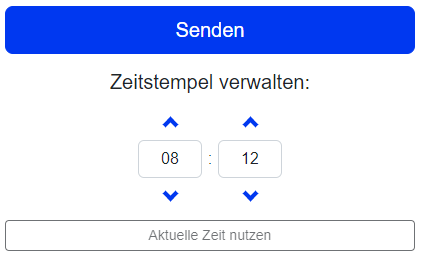
\includegraphics[width=.7\textwidth]{images/4-Feedback/time.png}
    \caption{Angepasste Eingabe der Updatezeit}
    \label{fig:feed-time}
\end{figure}

Dabei kann zwischen zwei Modi gewechselt werden.
Der als Standard ausgewählte Modus synchronisiert die Updatezeit stets mit der Systemzeit.
Hierzu wird die zu sehende digitale Uhr mit der aktuellen Uhrzeit synchronisiert.
Nach dem Absenden eines Updates wird die Zeit immer auf diese Einstellung zurückgesetzt.

Der zweite Modus kann für eine eigene Zeiteinstellung verwendet werden.
Hierzu kann die bestehende Uhrzeit entweder über die blauen Pfeile oder eine direkte Eingabe in die Eingabefelder geändert werden.
Sobald manuelle Änderungen an der Zeit festgestellt wurden wird die automatische Synchronisation gestoppt.
Möchten die Nutzenden zurück zur automatisiert synchronisierten Zeit zurückkehren, kann hierzu er untere Button "Aktuelle Zeit verwenden" geklickt werden.
Dieser ist nur aktiviert, solange die manuelle Zeiteingabe aktiv ist.

\textbf{Referenzieren von Updates:} Ebenfalls eingeführt wurde ein System zum Referenzieren von Updates.
Dieses ist jedoch auf eine Referenz pro Update beschränkt.
Wird auf den Link-Button in \autoref{fig:feed-timeline} geklickt, so wird dieses Update dem aktuellen Update als Referenz hinzugefügt.

\begin{figure}[htp]
    \centering
    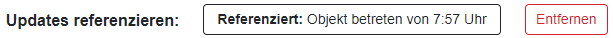
\includegraphics[width=\textwidth]{images/4-Feedback/reference.png}
    \caption{Referenzieren von Updates}
    \label{fig:feed-reference}
\end{figure}

Soll nun überprüft werden, welches Update momentan referenziert ist, kann auf die in \autoref{fig:feed-reference} zu sehenden Elemente geblickt werden.
Diese sind unter der Zeiteinstellung zu finden.
Das schwarz umrandete Feld zeigt dabei die Überschrift und die Zeit des referenzierten Updates an. Über den roten Button kann die Referenz entfernt werden.

\textbf{Letzte Standorte:} Dieses Feature wurde ebenfalls umgesetzt.
Dazu wird jeder verfügbaren Person in der Darstellung die Kennung ihres letzten Objekts in Klammern angehangen.

\textbf{Rechtschreibkorrektur:} Eine Rechtschreibkorrektur gestaltet sich als schwer umzusetzenden Feature.
Systeme für Rechtschreibkorrektur greifen stets auf Wortlisten zurück, welche auf externen Servern liegen.
Diese können aus dem internen Netzwerk des Finanzamts jedoch nicht angefragt werden.
Somit muss ein anderer Weg zur Umsetzung dieses Features gefunden werden.
Dies wurde jedoch auf einen späteren Zeitpunkt verlegt.
Vor Veröffentlichung der Software wird jedoch ein Rechtschreibkorrektur umgesetzt werden